\subsection{Encryption and Decryption}

Encryption is the transformation of message bits (\textit{plaintext}) into unintelligible form (\textit{ciphertext}) using mathematical formulas (encryption algorithm).
Only the intended recipient with the decryption algorithm can decrypt the ciphertext to see the original message \cite{Devi_2019}.
Figure \ref{fig:encryption-process.png} shows the encryption and decryption process.

\begin{figure}[!ht]
    \centering
    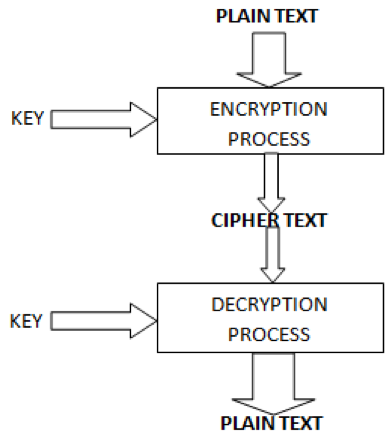
\includegraphics[width=.35\textwidth]{encryption-process.png}
    \caption{Encryption and decryption process \cite{Bhanot_2015}.}
    \label{fig:encryption-process.png}
\end{figure}


\subsubsection{Symmetric encryption}

Symmetric encryption algorithms use a single key that both the sender and recipient have.
This key is kept secret among sender and receiver so that no intruder can steal the data to be transferred by encrypting it  \cite{Bhanot_2015}.


\subsubsection{Asymmetric encryption}

Asymmetric encryption algorithm or public-key systems use two keys: a public key and a private key.
The public key is known to everyone while the private key is only used by the recipient of messages \cite{Bhanot_2015}.

Asymmetric encryption provides more security as compared to symmetric key encryption.
However, in case of encryption speed, symmetric encryption is on the lead \cite{Bhanot_2015}.

\subsubsection{Decryption Process}
\label{sec:decryption}

AES decryption is the process of reversing encryption steps to retrieve the original plaintext from a given ciphertext. Since AES is a symmetric block cipher, it uses the same secret key for both encryption and decryption\cite{NIST_AES}.

The input data is handled in 128-bit blocks and processed through multiple transformation rounds. The number of rounds depends on the key size: 10 rounds for 128-bit keys, 12 for 192-bit, and 14 for 256-bit keys.

To decrypt, AES performs the inverse of each encryption step, but in reverse order. These inverse operations are:

\begin{enumerate}
    \item \textbf{AddRoundKey}: This step XORs the block with the corresponding round key. Since XOR is its own inverse, this operation is identical in both encryption and decryption.
    \item \textbf{InvShiftRows}: Reverses the row shifts that were applied during encryption.
    \item \textbf{InvSubBytes}: Applies the inverse S-box substitution to each byte, undoing the non-linear transformation.
    \item \textbf{InvMixColumns}: Reverses the mixing of bytes in each column. This step is skipped in the final round.
\end{enumerate}

Decryption starts by XORing the ciphertext with the final round key. Then, each round applies the inverse transformations using the appropriate round key from the key schedule. After all rounds are completed, the original plaintext is recovered.
